\chapter{User interface design}\label{chapter:userInterfaceDesign}
\paragraph{}We have already dealt with the interface design in the Requirements Analysis and Specification Document, where we have shown some mock-ups of the screens of our applications.\\ In this section we will refine the user interface basically from the point of view of \textit{interaction} with the end-user (mapping between a sequence of actions and a screen flow).
\paragraph{} We will use the class diagram for the specification of screen flows. This approach need some clarification about the used notation:
\begin{table}[H]
\begin{longtable}{| p{0.3\textwidth} | p{0.7\textwidth} |}
\hline
\textbf{Symbol} & {\centering \textbf{Meaning}} \\ \hline
Directed arrow with \textit{function()} over it & It defines a transition from a particular user interface element to another. This transition is triggered by the invoking of a particular method \textit{function()} in the source interface element. \\ \hline
Class symbol & It determines a specific user interface element from the set \{\textit{Screen},\textit{Form},\textit{Element},\textit{Pop-up}\}
or a specific event (stereotype \textit{event}). In both cases the type of element is specified in the stereotype of the class symbol. \\ \hline
Composition symbol & Means that a specific user interface element is contained in another. Typically is used when a form or a list of elements is contained in a particular screen. \\ \hline
Directed arrow with the stereotype \textit{event} over it and a \textit{text} & Means that it is not a user induced function to trigger the transition, but an event from the software, in particular an event sent by the server to the client. The \textit{text} describe the event.\\ \hline
\end{longtable}
\caption{Notation for the user interface flow diagram}
\label{tab:userInterfaceDefinitions}
\end{table}
\section{Passenger App}
\begin{figure}[H]
	\centering
	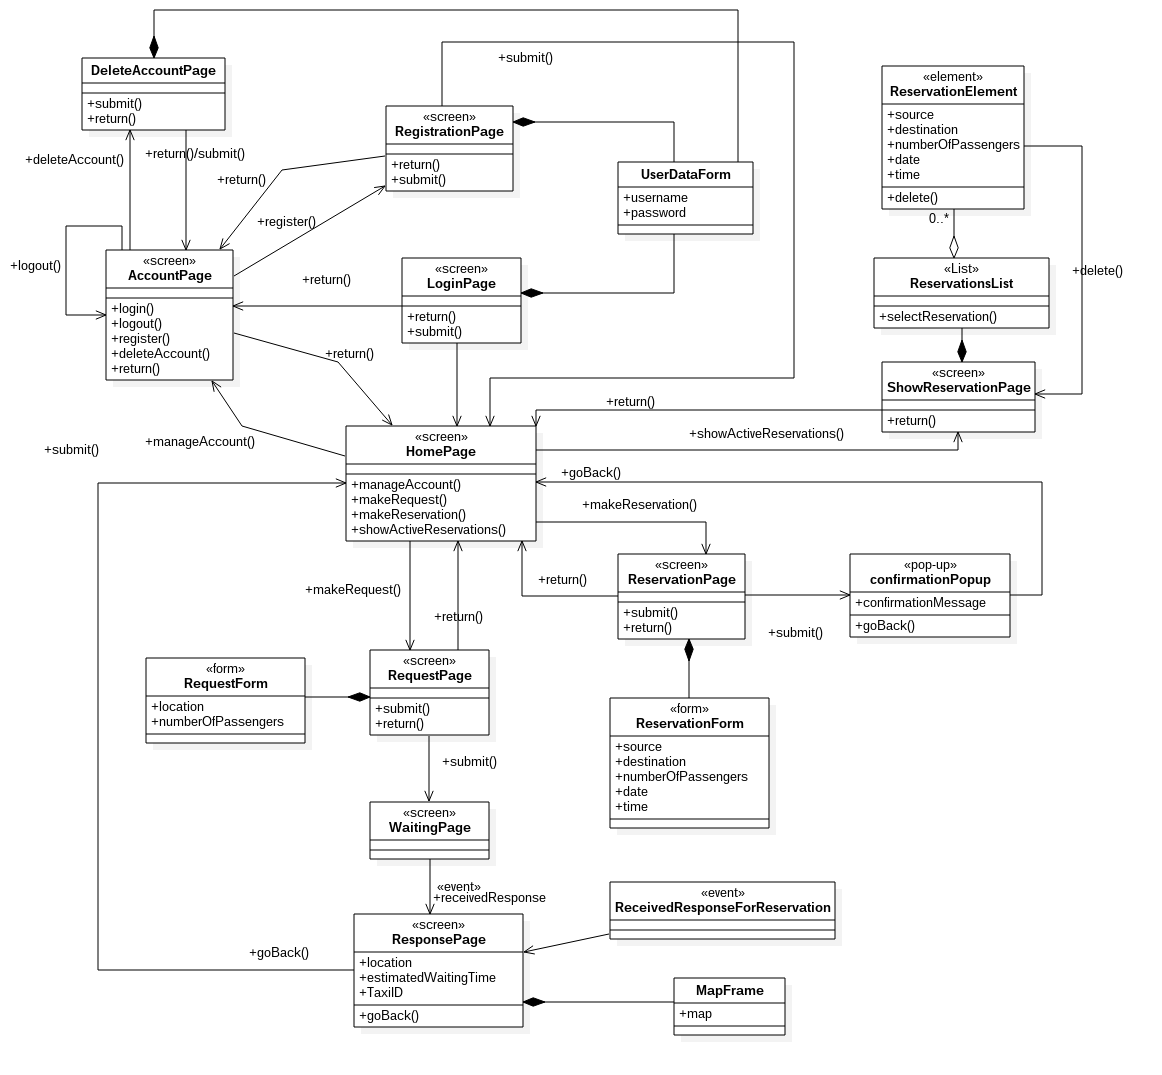
\includegraphics[trim= 100 0 0 0, scale=0.45]{../"Analysis Documents"/passengerApp_GUI}
	\caption{Screen flow of the Passenger mobile application}
	\label{fig:screenFlow:passengerApp}
\end{figure}
\section{Taxi Driver App}
\begin{figure}[H]
	\centering
	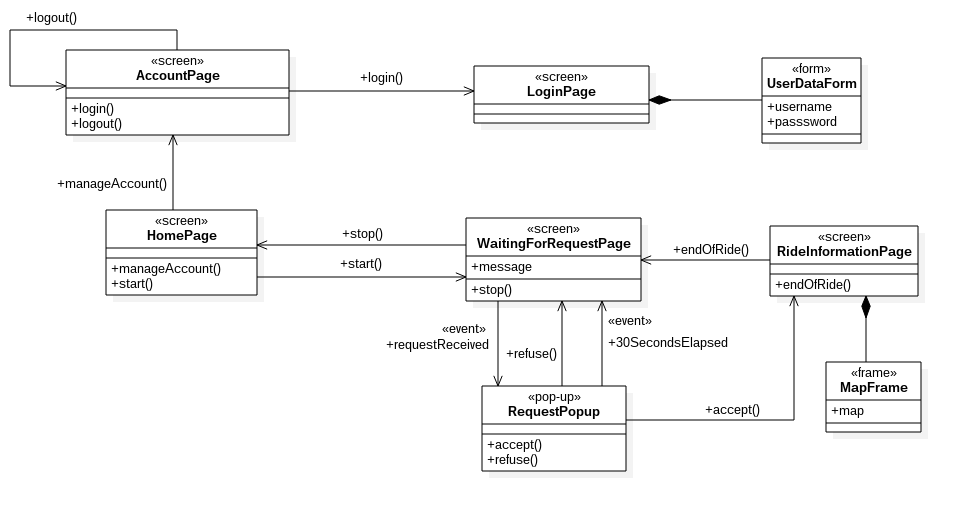
\includegraphics[trim = 50 0 0 0,scale=0.5]{../"Analysis Documents"/taxiDriverApp_GUI}
	\caption{Screen flow of the taxi driver mobile application}
	\label{fig:screenFlow:taxiDriverApp}
\end{figure}